% Copyright (c) 2014,2016,2018 Casper Ti. Vector
% Public domain.

\chapter{页缓存中数据预取的设计与实现}
%\pkuthssffaq % 中文测试文字。
\section{数据预取的设计}\label{sec:ra_design}
我们的数据预取的设计主要参考了 Linux 系统中的实现\parencite{readahead}。
做数据预取的目的是将磁盘 IO 的延迟对应用程序隐藏,达到应用程序的处理和磁盘 IO 并行的效果。
双窗口 (Dual Windows) 是一种常见的实现手段,可以达成流水线化的数据预取。
如图\ref{fig:readahead}所示,当应用程序在处理当前窗口 (current\_window) 中的数据时,
数据预取在预读窗口 (ahead\_window) 以后台的方式进行。
为了使这种应用程序和磁盘IO并行处理的状态能够延续,我们在 current\_window 中的某个页面上做标记 (lookahead\_index)。
当应用程序访问到带有标记的页面时,便会在预取窗口中触发新的数据预取。
当新的预取操作完成后,窗口会向前推进并在新的窗口内设置新的标记 new\_lookahead\_index。
如此循环往复,也就达到了我们最初的设计目的,表\ref{tab:readahead}总结了设计中的一些关键点。

\begin{figure}[h]
    \centering
    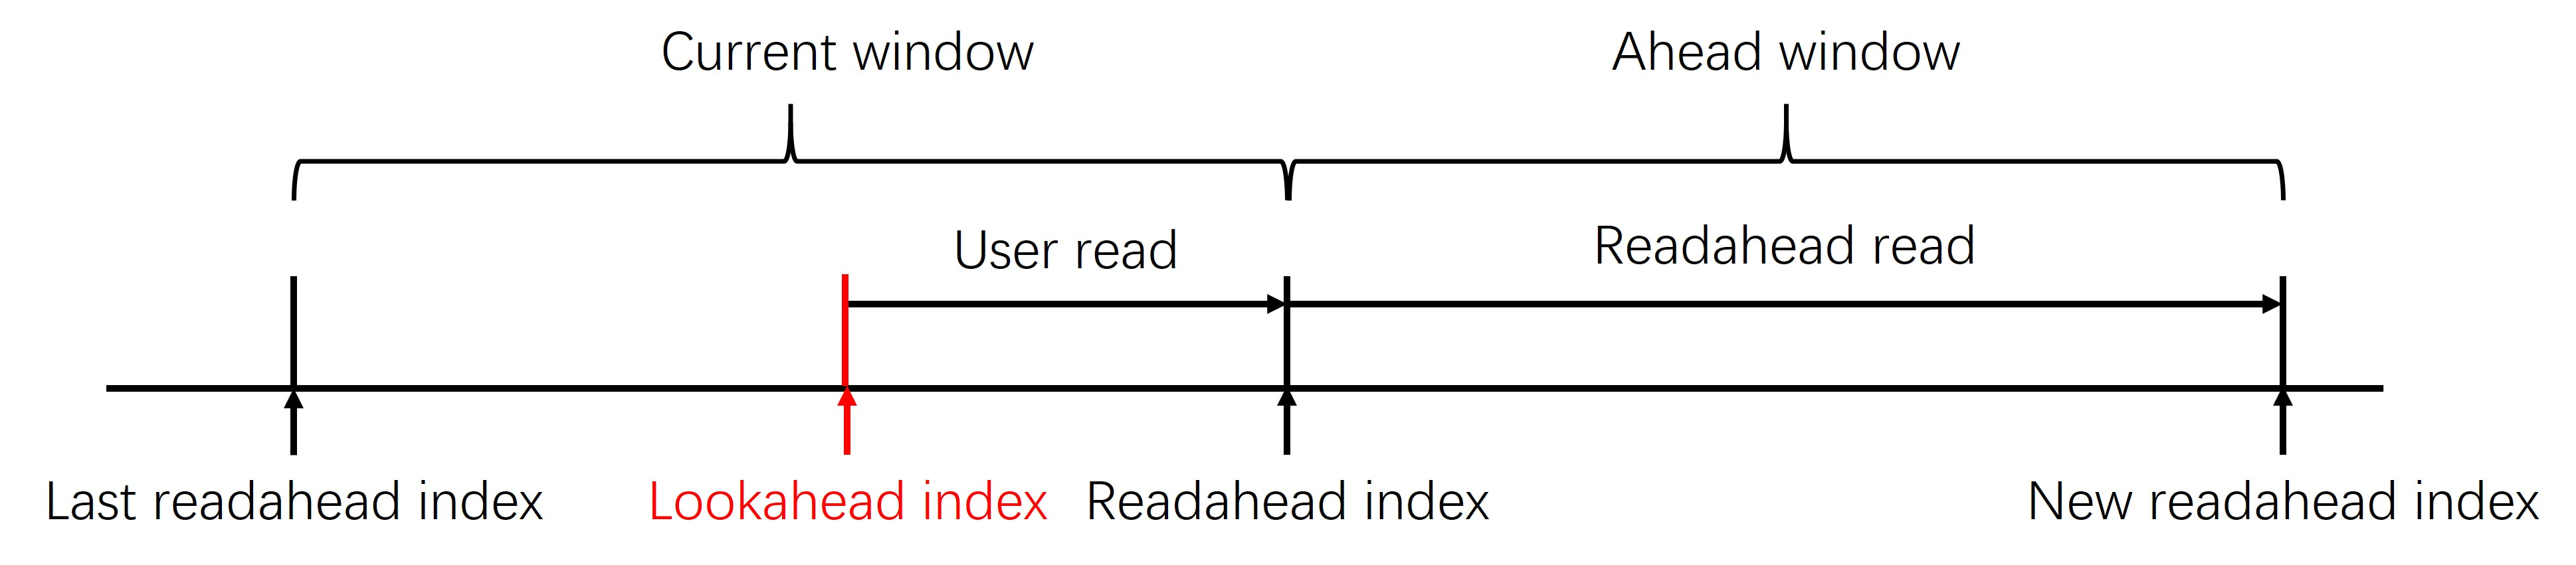
\includegraphics[width=1.0\textwidth]{chap4_readahead.jpg}
    \caption{数据预取行为示意}
    \label{fig:readahead}
\end{figure}

值得注意的一点是,考虑到数据预取对随机访问模式帮助不大,甚至还可能会起到负面效果,
我们的设计中会检测应用程序的访问模式,只对顺序访问模式做数据预取。
这就涉及到对顺序访问模式的检测,对此我们采用的是一种相对简单的方式:只考虑前一个访问的页面,
如果本次访问的页面编号和前一个访问的页面编号相差不超过1,就认为是本次访问是顺序访问。

\begin{table}[h]
    \centering
    \begin{tabularx}{\textwidth}{|c|Y|}
    \hline
    设计点 & 描述 \\
    \hline
    做预取的时机 & lookahead\_index \\
    \hline
    预取窗口 & readahead\_index .. readahead\_index + size \\
    \hline
    下次预取的时机 & new\_lookahead\_index \\
    \hline
    新的预取窗口 & new\_readahead\_index .. new\_ readahead\_index + new\_size 
                    (new\_readahead\_index = readahead\_index + size)\\
    \hline
    \end{tabularx}
    \caption{数据预取的关键点}
    \label{tab:readahead}
\end{table}

\section{数据预取的实现}
虽然数据预取的设计看起来非常简明,但还有一些实现的细节需要说明。

对于需要维护的状态,我们还是坚持以精简作为设计原则,不维护冗余信息。
为了实现\ref{sec:ra_design}节中的流水线化数据预取,至少需要维护预取窗口和标记页面。
另外,为了支持对应用访问模式的检测,还需要维护前一个访问的页面的编号。

关于预取窗口的长度的设置,我们的实现采用了倍增的方式进行调整。
窗口会被初始化为一个相对小的长度(我们选择了4个页面),随后窗口每向前推进一次,
将窗口大小翻倍,即 $ (offset, size) \Rightarrow (offset + size, 2*size) $。
考虑到底层设备的 IO 请求队列存在上限,为了避免单次请求包含过多的页面,
我们为窗口长度设置了一个上限,一旦达到上限就不再继续倍增。

还需要注明的一点是,设置 lookahead\_index 在当前窗口中的位置会影响到预读的效果。
在极端情况下,若设置 lookahead\_index 与 readahead\_index重合,流水线并行化的预取将退化为非并行的预取。
我们默认的设置方式是采用完全流水线并行化的方式,设置 lookahead\_index 为 last\_readahead\_index。

对于页缓存中的每个页面,有三种可能的状态:未初始化 (Uninit)、已同步 (Sync)、未同步(Dirty),
后两种状态统称为已初始化状态。
页缓存的数据预取属于异步读取,对于异步读取的处理方式一般是,先向存储设备提交读请求并将相关页面
的状态设置为 Uninit,待先前提交的请求完成时,将相关页面的状态更新为 Sync。
另外,为了避免向底层设备提交过多的请求,我们限制最多存在一个未完成的数据预取请求。

当上层向页缓存请求编号为 $ idx $ 的页面时,会调用 $ commit\_page(idx) $。
此时页缓存会首先查看先前提交的预取请求是否完成,如果请求完成,则更新相关页面的状态。
随后,页缓存处理当前访问编号为 $ idx $ 的页面的请求,这可能如下有三种情况。
\begin{itemize}
    \item 情况一:上层请求的页面在页缓存中,并处于已初始化状态。此时请求的页面已经可以返回,
    可以考虑是否提交新的数据预取请求。
    \item 情况二:上层请求的页面在页缓存中,并处于未初始化状态。此时请求的页面属于先前提交的数据预取请求,
    需等待请求的完成,并更新相关页面状态,再考虑是否提交新的数据预取请求。
    \item 情况三:上层请求的页面不在页缓存中。此时不得不做一个同步的读取操作读出请求的页面,
    再考虑是否提交新的数据预取请求。
\end{itemize}
若决定提交新的数据预取请求,则提交请求并初始化相关页面状态,否则直接返回上层请求的页面。

% vim:ts=4:sw=4
